\section{Capítulo 7 -- Busca}

Procurar é uma das tarefas que um programa mais repete: achar um cliente pelo CPF, um produto pelo código, uma palavra no dicionário, um contato na agenda. No Capítulo 2 você conheceu a busca sequencial e viu que ela é $O(n)$; no Capítulo 5, a árvore binária de busca, que encontra um valor descendo por um único caminho. Neste capítulo o foco é o vetor: você vai rever a busca sequencial, aprender a \textbf{busca binária}, que encontra um valor entre um milhão em apenas 20 comparações, e conhecer as variações e as funções prontas do C++ que todo programador usa no dia a dia.

\subsection{7.1 Busca sequencial}

A \textbf{busca sequencial} (ou linear) compara o valor procurado com cada elemento, do primeiro ao último, até encontrá-lo ou até o vetor acabar. É o que você faz ao procurar uma chave em uma gaveta bagunçada: olha uma por uma.

\begin{center}
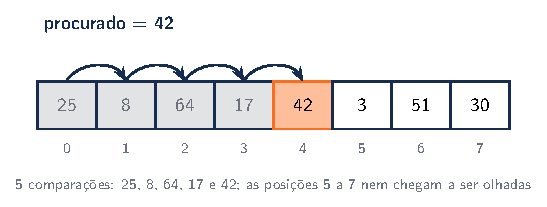
\includegraphics[width=0.8\linewidth,keepaspectratio]{imagens/capitulo-07_sequencial.pdf}
\end{center}

Sua grande vantagem é não exigir nada dos dados: o vetor pode estar em qualquer ordem, e o tipo dos elementos só precisa saber se comparar com \texttt{==}. Com um \textit{template} (Capítulo 1), a mesma função serve para números, textos e qualquer outro tipo. E, quando os elementos são registros, a busca costuma ser feita por uma \textbf{chave}, um campo que identifica o registro, como a matrícula de um aluno:

\begin{codigo}
\begin{Verbatim}[breaklines=true, breaksymbolleft={}, fontsize=\footnotesize]
#include <vector>

template <typename T>
int buscaSequencial(const vector<T> &v, const T &procurado) {
    for (int i = 0; i < static_cast<int>(v.size()); i++) {
        if (v[i] == procurado) return i;   // achou: para
    }
    return -1;                     // olhou todos e não achou
}

struct Aluno {
    int matricula;
    string nome;
};

// procura pela chave (a matrícula) e devolve o aluno inteiro
const Aluno *buscarAluno(const vector<Aluno> &turma,
                         int matricula) {
    for (const Aluno &a : turma) {
        if (a.matricula == matricula) return &a;
    }
    return nullptr;                // nenhum aluno com ela
}

int main() {
    vector<int> numeros = {25, 8, 64, 17, 42, 3, 51, 30};
    cout << buscaSequencial(numeros, 42) << endl;   // 4
    cout << buscaSequencial(numeros, 99) << endl;   // -1

    vector<string> cores = {"azul", "verde", "roxo"};
    cout << buscaSequencial(cores, string("roxo")) << endl; // 2

    vector<Aluno> turma = {{2031, "Ana"}, {1987, "Bruno"},
                           {2210, "Carla"}};
    const Aluno *achado = buscarAluno(turma, 1987);
    if (achado != nullptr) cout << achado->nome << endl; // Bruno
}
\end{Verbatim}
\end{codigo}

O \texttt{string("roxo")} é necessário porque \texttt{"roxo"} sozinho é um texto do C, e o \textit{template} precisa que os dois parâmetros sejam do mesmo tipo \texttt{T}. A função \texttt{buscarAluno} devolve um ponteiro para o aluno encontrado, ou \texttt{nullptr} quando não acha, o mesmo papel do $-1$ na versão com índices.

Como você viu no Capítulo 2, o melhor caso é uma comparação, o pior caso são $n$ comparações (o valor está no fim ou não existe) e o caso médio é cerca de $n/2$. A busca sequencial é $O(n)$.

\subsubsection{Duas melhorias simples}

Se o vetor estiver \textbf{ordenado}, a busca pode desistir mais cedo: ao encontrar um valor maior que o procurado, já se sabe que ele não está no resto do vetor. Isso não muda o pior caso, que continua $O(n)$, mas acelera as buscas sem sucesso.

A outra melhoria é a \textbf{sentinela}. O laço da busca sequencial faz duas perguntas a cada passo: ``o vetor acabou?'' e ``achei?''. Se o próprio valor procurado for colocado no fim do vetor, o laço com certeza vai parar nele, e a primeira pergunta deixa de ser necessária. No final, basta ver se o valor encontrado foi o verdadeiro ou a sentinela.

\begin{codigo}
\begin{Verbatim}[breaklines=true, breaksymbolleft={}, fontsize=\footnotesize]
#include <vector>

// vetor em ordem crescente: dá para desistir mais cedo
int buscaOrdenada(const vector<int> &v, int procurado) {
    for (int i = 0; i < static_cast<int>(v.size()); i++) {
        if (v[i] == procurado) return i;
        if (v[i] > procurado) return -1;   // o resto é maior
    }
    return -1;
}

// sentinela: uma comparação por passo em vez de duas
int buscaComSentinela(vector<int> &v, int procurado) {
    int n = static_cast<int>(v.size());
    v.push_back(procurado);       // garante que o laço para
    int i = 0;
    while (v[i] != procurado) i++;
    v.pop_back();                 // devolve o vetor como estava
    return i < n ? i : -1;        // parou na sentinela: não está
}
\end{Verbatim}
\end{codigo}

A sentinela economiza uma comparação por passo, o que pode fazer diferença em laços executados milhões de vezes, mas continua $O(n)$. Ela é um exemplo de otimização que melhora a constante, e não a ordem de crescimento.

\subsection{7.2 Busca binária}

Pense no jogo de adivinhar um número de 1 a 100, em que a cada palpite você ouve ``é maior'' ou ``é menor''. Ninguém joga chutando 1, 2, 3\ldots{} A estratégia natural é chutar 50: seja qual for a resposta, metade das possibilidades desaparece. Depois 25 ou 75, e assim por diante. Em no máximo 7 palpites você acerta.

A \textbf{busca binária} usa exatamente essa ideia em um vetor \textbf{ordenado}. Ela mantém uma faixa de posições onde o valor ainda pode estar, delimitada por \texttt{inicio} e \texttt{fim}, e a cada passo compara o procurado com o elemento do \textbf{meio} da faixa:

\begin{itemize}
  \item se for igual, achou;
  \item se o elemento do meio for \textbf{menor} que o procurado, o valor só pode estar à direita, e a faixa passa a começar em \texttt{meio + 1};
  \item se for \textbf{maior}, o valor só pode estar à esquerda, e a faixa passa a terminar em \texttt{meio - 1};
  \item se a faixa ficar vazia (\texttt{inicio > fim}), o valor não está no vetor.
\end{itemize}

\begin{center}
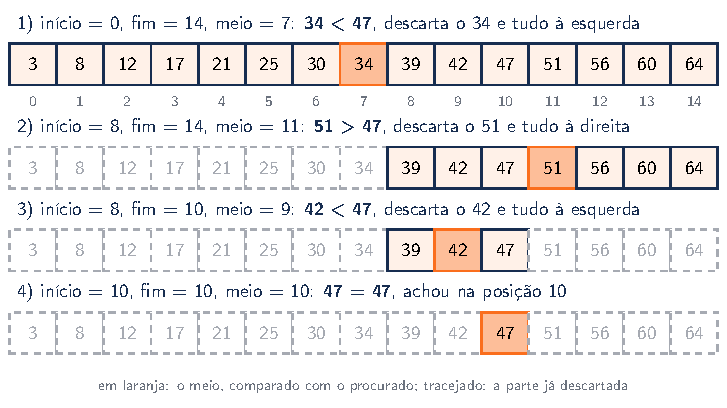
\includegraphics[width=\linewidth,keepaspectratio]{imagens/capitulo-07_binaria.pdf}
\end{center}

\begin{codigo}
\begin{Verbatim}[breaklines=true, breaksymbolleft={}, fontsize=\footnotesize]
// trecho
int buscaBinaria(const vector<int> &v, int procurado) {
    int inicio = 0;
    int fim = static_cast<int>(v.size()) - 1;
    while (inicio <= fim) {           // ainda há onde procurar
        int meio = inicio + (fim - inicio) / 2;
        if (v[meio] == procurado) return meio;
        if (v[meio] < procurado) {
            inicio = meio + 1;        // descarta a esquerda
        } else {
            fim = meio - 1;           // descarta a direita
        }
    }
    return -1;                        // a faixa ficou vazia
}
\end{Verbatim}
\end{codigo}

Acompanhar a busca em uma tabela, com os valores de cada variável a cada volta do laço, é a melhor forma de entendê-la. Veja o que acontece ao procurar o 20, que não está no vetor da figura:

\begin{center}
\begin{tabular}{@{}p{0.08\linewidth}p{0.1\linewidth}p{0.06\linewidth}p{0.08\linewidth}p{0.12\linewidth}p{0.32\linewidth}@{}}
\toprule
\rowcolor{headergray}
\tblheader{Passo} & \tblheader{início} & \tblheader{fim} & \tblheader{meio} & \tblheader{v[meio]} & \tblheader{Decisão} \\
\midrule
1 & 0 & 14 & 7 & 34 & 20 < 34: fim = 6 \\
\rowcolor{rowgray} 2 & 0 & 6 & 3 & 17 & 20 > 17: início = 4 \\
3 & 4 & 6 & 5 & 25 & 20 < 25: fim = 4 \\
\rowcolor{rowgray} 4 & 4 & 4 & 4 & 21 & 20 < 21: fim = 3 \\
-- & 4 & 3 & & & início > fim: não está \\
\bottomrule
\end{tabular}
\end{center}

Repare no valor final de \texttt{inicio}: 4, exatamente a posição em que o 20 deveria ser inserido para o vetor continuar ordenado, entre o 17 e o 21. Essa observação será útil na Seção 7.3.

\begin{destaque}{Por que não \texttt{(inicio + fim) / 2}?}
As duas fórmulas dão o mesmo meio, mas \texttt{inicio + fim} pode passar do maior valor que um \texttt{int} guarda (cerca de 2,1 bilhões) em vetores muito grandes, e o resultado vira um número negativo. Já \texttt{inicio + (fim - inicio) / 2} nunca passa de \texttt{fim}. Esse erro ficou escondido por anos na busca binária da biblioteca do Java, até ser descoberto em 2006, quando os vetores ficaram grandes o bastante para ele aparecer.
\end{destaque}

\subsubsection{Versão recursiva}

A busca binária também tem uma definição recursiva natural, como os percursos de árvore do Capítulo 5: o caso base é a faixa vazia, e cada chamada procura em uma das metades.

\begin{codigo}
\begin{Verbatim}[breaklines=true, breaksymbolleft={}, fontsize=\footnotesize]
// trecho
int buscaBinariaRecursiva(const vector<int> &v, int procurado,
                          int inicio, int fim) {
    if (inicio > fim) return -1;      // caso base: faixa vazia
    int meio = inicio + (fim - inicio) / 2;
    if (v[meio] == procurado) return meio;
    if (v[meio] < procurado) {
        return buscaBinariaRecursiva(v, procurado, meio + 1, fim);
    }
    return buscaBinariaRecursiva(v, procurado, inicio, meio - 1);
}
\end{Verbatim}
\end{codigo}

As duas versões fazem as mesmas comparações. A iterativa é a mais usada na prática, porque não gasta a pilha de execução; a recursiva é mais próxima da definição e aparece muito em provas. Este é o programa completo com as duas:

\begin{codigo}
\begin{Verbatim}[breaklines=true, breaksymbolleft={}, fontsize=\footnotesize]
#include <vector>

int buscaBinaria(const vector<int> &v, int procurado) {
    int inicio = 0;
    int fim = static_cast<int>(v.size()) - 1;
    while (inicio <= fim) {           // ainda há onde procurar
        int meio = inicio + (fim - inicio) / 2;
        if (v[meio] == procurado) return meio;
        if (v[meio] < procurado) {
            inicio = meio + 1;        // descarta a esquerda
        } else {
            fim = meio - 1;           // descarta a direita
        }
    }
    return -1;                        // a faixa ficou vazia
}

int buscaBinariaRecursiva(const vector<int> &v, int procurado,
                          int inicio, int fim) {
    if (inicio > fim) return -1;      // caso base: faixa vazia
    int meio = inicio + (fim - inicio) / 2;
    if (v[meio] == procurado) return meio;
    if (v[meio] < procurado) {
        return buscaBinariaRecursiva(v, procurado, meio + 1, fim);
    }
    return buscaBinariaRecursiva(v, procurado, inicio, meio - 1);
}

int main() {
    vector<int> v = {3, 8, 12, 17, 21, 25, 30, 34, 39, 42,
                     47, 51, 56, 60, 64};
    cout << buscaBinaria(v, 47) << endl;            // 10
    cout << buscaBinaria(v, 20) << endl;            // -1
    cout << buscaBinaria(v, 3) << " "
         << buscaBinaria(v, 64) << endl;            // 0 14
    int ultimo = static_cast<int>(v.size()) - 1;
    cout << buscaBinariaRecursiva(v, 47, 0, ultimo) << endl; // 10
}
\end{Verbatim}
\end{codigo}

\subsubsection{Quanto custa}

Cada comparação descarta metade da faixa: de $n$ posições sobram $n/2$, depois $n/4$, $n/8$\ldots{} até sobrar uma. O número de passos é quantas vezes $n$ pode ser dividido por 2, ou seja, $\log_2 n$. A busca binária é $O(\log n)$, e é isso que a torna tão poderosa:

\begin{center}
\begin{tabular}{@{}p{0.3\linewidth}p{0.32\linewidth}p{0.28\linewidth}@{}}
\toprule
\rowcolor{headergray}
\tblheader{Tamanho do vetor} & \tblheader{Sequencial (pior caso)} & \tblheader{Binária (pior caso)} \\
\midrule
15 & 15 comparações & 4 comparações \\
\rowcolor{rowgray} 1.000 & 1.000 & 10 \\
1.000.000 & 1.000.000 & 20 \\
\rowcolor{rowgray} 1.000.000.000 & 1.000.000.000 & 30 \\
\bottomrule
\end{tabular}
\end{center}

Multiplicar o vetor por mil acrescenta só 10 comparações. Mas a busca binária cobra um preço: o vetor precisa estar \textbf{ordenado}, e precisa permitir acesso direto a qualquer posição. Em uma lista encadeada (Capítulo 3), chegar ao meio já custa $O(n)$, e a vantagem desaparece.

\subsection{7.3 Variações da busca binária}

A busca binária básica responde ``está ou não está?''. Com pequenas mudanças, ela responde perguntas mais úteis.

\subsubsection{Primeira ocorrência e ponto de inserção}

Quando o vetor tem valores repetidos, a busca básica devolve a posição de \textbf{algum} deles, não necessariamente a do primeiro. A variação abaixo encontra a \textbf{primeira posição com valor maior ou igual} ao procurado. Se o valor existe, é a sua primeira ocorrência; se não existe, é a posição onde ele deveria ser inserido.

A diferença está no tratamento do meio: quando \texttt{v[meio]} é maior ou igual ao procurado, o meio ainda pode ser a resposta, então a faixa passa a terminar \textbf{nele} (\texttt{fim = meio}), em vez de descartá-lo. Para isso funcionar, \texttt{fim} começa fora do vetor, em \texttt{v.size()}, e o laço para quando \texttt{inicio} e \texttt{fim} se encontram.

Com ela, contar quantas vezes um valor aparece também fica $O(\log n)$: é a distância entre a primeira posição do valor e a primeira posição do valor seguinte.

\subsubsection{Busca binária na resposta}

A busca binária não precisa de um vetor. Ela funciona em qualquer faixa de números em que uma pergunta tenha resposta ``sim'' até certo ponto e ``não'' daí em diante. Um exemplo é a raiz quadrada inteira de $n$: o maior $x$ tal que $x^2 \le n$. Para $x = 0, 1, 2, \ldots$, a resposta a ``$x^2 \le n$?'' é sim, sim, sim\ldots{} e depois sempre não. A busca binária encontra o último ``sim'' sem testar um por um.

\begin{codigo}
\begin{Verbatim}[breaklines=true, breaksymbolleft={}, fontsize=\footnotesize]
#include <vector>

// primeira posição com valor >= procurado
// (v.size() se todos forem menores)
int primeiraPosicao(const vector<int> &v, int procurado) {
    int inicio = 0;
    int fim = static_cast<int>(v.size());  // fora do vetor
    while (inicio < fim) {
        int meio = inicio + (fim - inicio) / 2;
        if (v[meio] < procurado) {
            inicio = meio + 1;     // a resposta está à direita
        } else {
            fim = meio;            // o meio ainda pode ser ela
        }
    }
    return inicio;
}

int contar(const vector<int> &v, int valor) {
    return primeiraPosicao(v, valor + 1)
           - primeiraPosicao(v, valor);
}

// maior x tal que x * x <= n
long long raizInteira(long long n) {
    long long inicio = 1, fim = n, resposta = 0;
    while (inicio <= fim) {
        long long meio = inicio + (fim - inicio) / 2;
        if (meio <= n / meio) {    // meio * meio <= n sem estouro
            resposta = meio;       // serve; tenta um maior
            inicio = meio + 1;
        } else {
            fim = meio - 1;        // grande demais
        }
    }
    return resposta;
}

int main() {
    vector<int> notas = {4, 5, 5, 7, 7, 7, 8, 9, 10};
    cout << primeiraPosicao(notas, 7) << endl;  // 3: 1º 7
    cout << primeiraPosicao(notas, 6) << endl;  // 3: entraria
    cout << primeiraPosicao(notas, 11) << endl; // 9: no fim
    cout << contar(notas, 7) << " "
         << contar(notas, 6) << endl;            // 3 0

    cout << raizInteira(50) << " "
         << raizInteira(1000000) << endl;        // 7 1000
    cout << raizInteira(1000000000000) << endl;  // 1000000
}
\end{Verbatim}
\end{codigo}

Na \texttt{raizInteira}, a comparação \texttt{meio <= n / meio} evita calcular \texttt{meio * meio}, que estouraria até um \texttt{long long} com $n$ na casa do trilhão. A mesma técnica resolve problemas como ``qual o menor tamanho de página que faz o texto caber em 10 páginas?'' ou ``qual a menor velocidade que permite terminar a entrega a tempo?'': sempre que a resposta pode ser testada e o teste muda de ``não'' para ``sim'' uma única vez.

\subsection{7.4 Busca na biblioteca padrão}

Na prática, você raramente vai escrever essas buscas do zero: o C++ traz todas elas prontas na biblioteca \texttt{<algorithm>}. Elas trabalham com \textbf{iteradores}, que indicam posições: \texttt{v.begin()} é o início do vetor e \texttt{v.end()} é a posição logo depois do último. Subtrair \texttt{v.begin()} de um iterador dá o índice.

\begin{codigo}
\begin{Verbatim}[breaklines=true, breaksymbolleft={}, fontsize=\footnotesize]
#include <vector>
#include <algorithm>   // find, sort, lower_bound...

int main() {
    vector<int> v = {25, 8, 64, 17, 42, 3, 51, 30};
    auto it = find(v.begin(), v.end(), 42);    // sequencial: O(n)
    if (it != v.end()) {
        cout << "posição " << it - v.begin() << endl; // 4
    }

    sort(v.begin(), v.end());           // 3 8 17 25 30 42 51 64
    cout << boolalpha
         << binary_search(v.begin(), v.end(), 42) << endl; // true

    auto p = lower_bound(v.begin(), v.end(), 20);  // 1º >= 20
    cout << *p << " na posição " << p - v.begin() << endl;
    // 25 na posição 3

    vector<int> notas = {4, 5, 5, 7, 7, 7, 8, 9, 10};
    auto [primeiro, depois] =
        equal_range(notas.begin(), notas.end(), 7);
    cout << depois - primeiro << " notas 7" << endl;  // 3 notas 7
}
\end{Verbatim}
\end{codigo}

\begin{center}
\begin{tabular}{@{}p{0.25\linewidth}p{0.17\linewidth}p{0.5\linewidth}@{}}
\toprule
\rowcolor{headergray}
\tblheader{Função} & \tblheader{Custo} & \tblheader{Devolve} \\
\midrule
\texttt{find} & $O(n)$ & iterador para o elemento, ou \texttt{end()} se não achar \\
\rowcolor{rowgray} \texttt{binary\_search} & $O(\log n)$ & \texttt{true} ou \texttt{false} \\
\texttt{lower\_bound} & $O(\log n)$ & primeira posição com valor $\ge$ procurado \\
\rowcolor{rowgray} \texttt{upper\_bound} & $O(\log n)$ & primeira posição com valor $>$ procurado \\
\texttt{equal\_range} & $O(\log n)$ & o par (\texttt{lower\_bound}, \texttt{upper\_bound}) \\
\bottomrule
\end{tabular}
\end{center}

A \texttt{lower\_bound} é a \texttt{primeiraPosicao} da Seção 7.3. Todas as funções de busca binária supõem que o vetor já está ordenado; se não estiver, elas não acusam erro nenhum, apenas devolvem respostas erradas. A \texttt{sort} usada no exemplo ordena o vetor em $O(n \log n)$; o Capítulo 8 mostra como algoritmos assim funcionam por dentro.

\subsection{7.5 Qual busca usar}

Se a busca binária é tão mais rápida, por que não usá-la sempre? Porque ordenar também custa. Ordenar um vetor de um milhão de elementos custa algo como $n \log_2 n \approx 20$ milhões de operações, muito mais que uma única busca sequencial (um milhão). A conta muda quando o mesmo vetor é consultado muitas vezes:

\begin{center}
\begin{tabular}{@{}p{0.2\linewidth}p{0.32\linewidth}p{0.4\linewidth}@{}}
\toprule
\rowcolor{headergray}
\tblheader{Buscas} & \tblheader{Só sequencial} & \tblheader{Ordenar uma vez + binária} \\
\midrule
1 & 1 milhão & 20 milhões + 20 \\
\rowcolor{rowgray} 100 & 100 milhões & 20 milhões + 2 mil \\
1 milhão & 1 trilhão & 20 milhões + 20 milhões \\
\bottomrule
\end{tabular}
\end{center}

Para uma busca isolada, a sequencial ganha; a partir de umas poucas dezenas de buscas no mesmo vetor, ordenar compensa com folga. A escolha também depende de quanto os dados mudam. Manter um vetor ordenado custa caro: cada inserção precisa deslocar os elementos maiores para abrir espaço. Por isso existem estruturas feitas para buscar e inserir rápido ao mesmo tempo:

\begin{center}
\begin{tabular}{@{}p{0.42\linewidth}p{0.24\linewidth}p{0.26\linewidth}@{}}
\toprule
\rowcolor{headergray}
\tblheader{Estrutura} & \tblheader{Buscar} & \tblheader{Inserir} \\
\midrule
vetor fora de ordem & $O(n)$ & $O(1)$ no fim \\
\rowcolor{rowgray} vetor ordenado & $O(\log n)$ & $O(n)$ \\
lista encadeada (Capítulo 3) & $O(n)$ & $O(1)$ no início \\
\rowcolor{rowgray} árvore AVL (Capítulo 5) & $O(\log n)$ & $O(\log n)$ \\
tabela hash (\texttt{unordered\_map}) & $O(1)$ em média & $O(1)$ em média \\
\bottomrule
\end{tabular}
\end{center}

Resumindo: poucos dados ou uma busca só, use a sequencial; dados que mudam pouco e são muito consultados, ordene e use a binária; dados que mudam e são consultados o tempo todo, use uma árvore balanceada (o \texttt{set} e o \texttt{map} do C++) ou uma tabela hash (o \texttt{unordered\_set} e o \texttt{unordered\_map}), que encontra uma chave em tempo médio constante calculando, a partir da própria chave, a posição onde ela está guardada.

\begin{destaque}{Comparando com Python}
Em Python, o operador \texttt{in} e o método \texttt{index} das listas fazem busca sequencial, $O(n)$. A busca binária está no módulo \texttt{bisect}: \texttt{bisect\_left} é a \texttt{lower\_bound} do C++ e \texttt{bisect\_right} é a \texttt{upper\_bound}.

\begin{codigo}
\begin{Verbatim}[breaklines=true, breaksymbolleft={}, fontsize=\footnotesize]
from bisect import bisect_left, bisect_right

numeros = [3, 8, 12, 17, 21, 25, 30, 34, 39, 42,
           47, 51, 56, 60, 64]
print(42 in numeros)        # True: busca sequencial
print(numeros.index(42))    # 9

def busca_binaria(v, procurado):
    inicio, fim = 0, len(v) - 1
    while inicio <= fim:
        meio = (inicio + fim) // 2
        if v[meio] == procurado:
            return meio
        if v[meio] < procurado:
            inicio = meio + 1
        else:
            fim = meio - 1
    return -1

print(busca_binaria(numeros, 47))   # 10

notas = [4, 5, 5, 7, 7, 7, 8, 9, 10]
print(bisect_left(notas, 7))                            # 3
print(bisect_right(notas, 7) - bisect_left(notas, 7))   # 3
\end{Verbatim}
\end{codigo}

Como os inteiros do Python não têm limite, \texttt{(inicio + fim) // 2} não estoura. Repare no \texttt{//}, a divisão inteira: com \texttt{/}, o resultado seria um \texttt{float} e não serviria de índice. Para buscar muitas vezes por chave, o Python usa o \texttt{set} e o \texttt{dict}, que são tabelas hash: \texttt{42 in conjunto} é $O(1)$ em média, enquanto \texttt{42 in lista} é $O(n)$.
\end{destaque}

\subsection{Erros Comuns}

\begin{itemize}
  \item \textbf{Usar a busca binária em um vetor fora de ordem.} Ela não acusa erro: simplesmente descarta a metade errada e responde que o valor não está lá, mesmo quando está.
  \item \textbf{Errar a condição do laço.} Com \texttt{inicio} e \texttt{fim} apontando para posições válidas, o laço é \texttt{while (inicio <= fim)}. Com \texttt{<}, a busca deixa de olhar a última posição que sobrou.
  \item \textbf{Não descartar o meio.} Escrever \texttt{inicio = meio} em vez de \texttt{inicio = meio + 1} pode fazer a faixa parar de diminuir, e o laço nunca termina.
  \item \textbf{Calcular o meio com \texttt{(inicio + fim) / 2}} em vetores enormes. A soma pode estourar o \texttt{int}; use \texttt{inicio + (fim - inicio) / 2}.
  \item \textbf{Esperar a primeira ocorrência da busca básica.} Com valores repetidos, ela devolve um deles, não necessariamente o primeiro. Para o primeiro, use a \texttt{lower\_bound}.
  \item \textbf{Usar a busca binária em uma lista encadeada.} Sem acesso direto às posições, chegar ao meio já custa $O(n)$.
  \item \textbf{Ordenar o vetor para fazer uma única busca.} A ordenação custa mais que a própria busca sequencial; só compensa quando o vetor é consultado muitas vezes.
  \item \textbf{Esquecer de conferir o resultado de \texttt{find} e \texttt{lower\_bound}.} Se o valor não existir, elas devolvem \texttt{end()}, e usar \texttt{*it} nesse caso acessa uma posição fora do vetor.
\end{itemize}
